\documentclass[t]{beamer}

\mode<presentation>
{
  \usetheme{CambridgeUS}  % or try Darmstadt, Madrid, Warsaw, CambridgeUS ...
  \usecolortheme{default} % or try albatross, beaver, crane, ...
  \usefonttheme{default}  % or try serif, structurebold, ...
  \setbeamertemplate{navigation symbols}{}
  \setbeamertemplate{caption}[numbered]
} 

\usepackage[english]{ babel }
\usepackage[utf8x]{ inputenc }
\usepackage{ physics }
\usepackage{ bbold }
\usepackage{ multicol }
\usepackage{caption}
\usepackage{graphicx}
\usepackage{mathtools}
\usepackage{comment}


\usepackage{tikz}
\usetikzlibrary{arrows}


\title[Holonomic Optimal Control for Qudits]{Holonomic Optimal Control for Qudits}
% Efficient (Scheme for) Non-adiabatic Holonomic Single-Qudit Gates with/using Dark Paths
\author{ Tomas André} \\ {\scriptsize \textit{Supervisor: Erik Sjöqvist \\ Subject reader: Martin Almquist}}
\
\institute{ Uppsala University }

\date{\today}
	
\begin{document}

\begin{frame}
  \titlepage
\end{frame}

%%%%%%%%%%%%%%%%%%%%%%%%%%%%%%%%%%%%%%%%%%%%%%%%%%%%

\section{Introduction}
\begin{frame}{Outline}
\tableofcontents
\end{frame}

\begin{frame}{}
\tableofcontents[ 
currentsubsection, 
hideothersubsections, 
sectionstyle=show/shaded, 
subsectionstyle=show/shaded, 
] 
\end{frame}
%
%\begin{frame}[c]{Motivation}
%''Nature isn't classical, dammit, and if you want to make a simulation of nature, you'd better make it quantum mechanical, and by golly it's a wonderful problem, because it doesn't look so easy.'' 
%\\- Richard Feynman
%\end{frame}

\begin{comment}


\begin{frame}{History (1/2)}
\begin{itemize}
\item[1980] Paul Benioff proposes a quantum mechanical model of the turing machine. 
\footnote{{\scriptsize Benioff, Paul (1980). Journal of Statistical Physics.22(5):563.}}


\item[1980s] Both Richard Feynman and Yuri Manin suggests that a quantum based computer could perform calculations not possible on a conventional computer.
\footnote{\scriptsize Feynman, Richard (June 1982). International Journal of Theoretical Physics. 21(6/7):467.}
\footnote{\scriptsize Manin, Yu. I. (1980). Vychislimoe i nevychislimoe [Computable and Noncomputable]}


\item[1994] Peter Shor publishes a quantum algorithm used for finding the prime-factors of an integer.
\footnote{\scriptsize Shor, Peter (1994). IEEE Comput Soc Press:p.124} (This is big!) 
\end{itemize}
\end{frame}

\begin{frame}{History (2/2)}

\begin{itemize}
\item[1998] The first two-qubit quantum computer capable of running calculations is built by Isaac Chaung, Neil Gershenfeld and Mark Kubinec. 
\footnote{\scriptsize Chuang, Isaac L.; Gershenfeld, Neil; Kubinec, Markdoi(1998). Phys. Rev. Lett. American Physical Society. 80(15):3408.}

\item[2001] IBM uses the Shor algorithm to factor the integer 15. \footnote{BM Research Division. "IBM's Test-Tube Quantum Computer Makes History; First Demonstration Of Shor's Historic Factoring Algorithm." ScienceDaily. (dec 2001)}

\item[2019] Google claims to have achieved computations on a quantum machine that would be infeasible on a classical computer.  
\footnote{\scriptsize Gibney, Elizabeth (October 2019). Nature. 574(7779):461.}


\item[Today] Both IBM and Google have active QC research and IBM has a quantum computer with 127 qubits. Despite much focus, fault tolerant quantum computers are still a far way off.

\end{itemize}
\end{frame}
\end{comment}


\begin{frame}{Quantum Computing (QC)}
\begin{block}{What is Quantum Computation?}
\begin{itemize}
\item Using quantum systems to perform computations instead of classical systems
\item Taking advantage of quantum mechanical effects for computational purposes
    
\item Utilizes \textbf{qubits} instead of bits
\begin{equation}
   \ket{\psi} = \alpha\ket{0} + \beta\ket{1} \Dot{=} \begin{pmatrix}
   \alpha\\ \beta 
   \end{pmatrix},\, |\alpha|^2 + |\beta|^2 = 1,\, \alpha,\beta\in\mathbb{C}
\end{equation}

\end{itemize}
\end{block}

\begin{block}{Higher dimensional computational elements}
\begin{itemize}
    \item bit $0,1 \;\mapsto$ qubit 
    \item trit $0,1,2 \;\mapsto$ qutrit   
    \item dit  $0,1,\dots, d \;\mapsto$ qudit
\end{itemize}
\end{block}
    
\end{frame}



\begin{comment}
\begin{frame}{What is computation?}

\begin{figure}
\includegraphics[scale=0.4]{dia1.png}
\end{figure}

\end{frame}


\begin{frame}{What is computation?}

\begin{figure}
\includegraphics[scale=0.4]{dia2.png}
\end{figure}

\end{frame}

\end{comment}






\section{Geometric Quantum Computation}

\begin{frame}{}
\tableofcontents[ 
currentsubsection, 
hideothersubsections, 
sectionstyle=show/shaded, 
subsectionstyle=show/shaded, 
] 
\end{frame}

\begin{frame}{Computation from Geometry}
\begin{figure}
\begin{center}
\includegraphics[scale=0.25]{geom.png}
\captionsetup{labelformat=empty}
\caption{{\tiny Image credit: Lloyd, Seth (june 2001)."Computation From Geometry". Science vol. 292}}
\end{center}
\end{figure}
\end{frame}

% FUCK THIS SLIDE
%\begin{frame}{Holonomies (1/2)}
%
%The change of a quantum state is called time-evolution, during one period of time $T$ it is written $U(T,0)$.
%
%The Berry phase is an early example a 1D Holonomy in Quantum mechanics.\footnote{\scriptsize Berry, Michael. Proceedings of the Royal Society of London. Series A, Mathematical and Physical Sciences. vol. 392 (June 1983).}
%\begin{equation}
%\ket{\psi(t)} \xrightarrow{\text{time passes}} \ket{\psi(t+T)} = e^{i(\theta + \gamma)}\ket{\psi(t)}
%\end{equation}
%in this case
%\begin{equation}
%U(0,T) = e^{i(\theta + \gamma)}
%\end{equation}
%
%$\theta$ - dynamical phase, arises from the Hamiltonian of the system.\\
%$\gamma$ - 'berry phase', or geometric phase arises from the geometry of the 'landscape'.
%\end{frame}


\begin{frame}{Holonomies (1/2)}
\begin{figure}
\begin{center}
\includegraphics[scale=6]{presentation/Connection-on-sphere.png}
\captionsetup{labelformat=empty}
\caption{{\tiny Image credit: Fjung at en.wikipedia: https://commons.wikimedia.org/w/index.php?curid=5126050}}
\end{center}
\end{figure}

\end{frame}


\begin{frame}{Holonomies (2/2)}
More generally a holonomy can be higher dimensional and non-abelian (matrix)
\begin{equation}
U(T,0) = \mathcal{T}\exp\left(i\int_{0}^{T} \underbrace{\mathbf{A}(t)}_{\text{Geometric}} - \underbrace{\mathbf{H}(t)}_{\text{Dynamic}}\,dt\right)
\end{equation}
where $\mathbf{A}_{mn}(t) = i\bra{m(t)}\pdv{}{t}\ket{n(t)}$ and
$\mathbf{H}_{mn}(t) = \bra{m(t)}\mathbf{H}(t)\ket{n(t)}$.
In the non-adiabatic case one wishes to remove dynamical phase contribution, then one is left with the Wilczek-Zee holonomy\footnote{F. Wilczek and A. Zee. Physical Review Letters. vol. 52. (1984)};
\begin{equation}
U(T,0) = \mathcal{T}\exp\left(i\int_{0}^{T}\mathbf{A}(t)\,dt\right) = \mathcal{P}\exp\left(i\oint_{C}\mathbf{A}(s)\,ds\right) = U(C)
\end{equation}
\end{frame}


\section{Results}

\begin{frame}{}
\tableofcontents[ 
currentsubsection, 
hideothersubsections, 
sectionstyle=show/shaded, 
subsectionstyle=show/shaded, 
] 
\end{frame}

\subsection{The qutrit}
\begin{frame}{}
\tableofcontents[ 
currentsubsection, 
hideothersubsections, 
sectionstyle=show/shaded, 
subsectionstyle=show/shaded, 
] 
\end{frame}

\begin{frame}{Designing the system}

The idea is the extension of a qubit implemented in a $^{171}$Yb$^{+}$ ion\footnote{\scriptsize MZ. Ai, S. Li, R. He, ZY. Xue, JM. Cui, YF. Haung, CF. Li, GC. Guo Experimental Realization of Nonadiabatic Holonomic
Single-Qubit Quantum Gates with Two Dark Paths in a
Trapped Ion}.
This project is limited to the quantum mechanical models.

% USE BLACKBOARD
% Draw the qubit system and explain how it extends
\end{frame}


\begin{frame}{Designing the system}

\begin{figure}[H]
    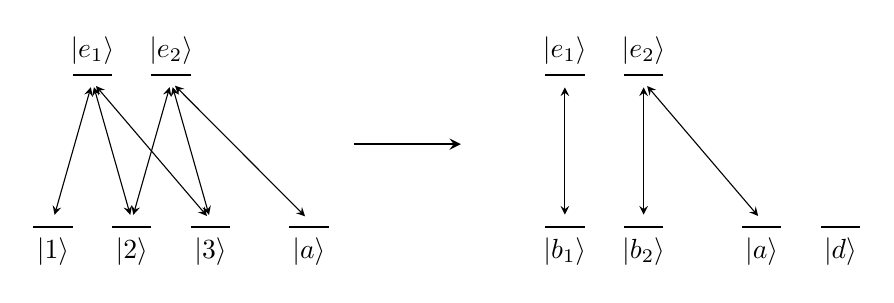
\begin{tikzpicture}[
      scale=0.5,
      level/.style={thick},
      virtual/.style={thick,densely dashed},
      trans/.style={thin,<->,shorten >=2pt,shorten <=2pt,>=stealth},
      arrow/.style={thick,->,shorten >=2pt,shorten <=2pt,>=stealth},
      classical/.style={thin,double,<->,shorten >=4pt,shorten <=4pt,>=stealth}]
      
    % Excited
    \draw[level] (5cm,0em) -- (6cm,0em) node[midway,above] {$\ket{e_1}$};    
    \draw[level] (7cm,0em) -- (8cm,0em) node[midway,above] {$\ket{e_2}$};
	% Ground states
    \draw[level] (4cm,-11em) -- (5cm,-11em) node[midway,below] {$\ket{1}$};
    \draw[level] (6cm,-11em) -- (7cm,-11em) node[midway,below] {$\ket{2}$};
    \draw[level] (8cm,-11em) -- (9cm,-11em) node[midway,below] {$\ket{3}$};
    \draw[level] (10.5cm,-11em) -- (11.5cm,-11em) node[midway,below] {$\ket{a}$};
    % e_1
    % Draw the transitions.
    \draw[trans] (5.5cm,-0.5em) -- (4.5cm,-10.5em) node[midway,left] {};
    \draw[trans] (5.5cm,-0.5em) -- (6.5cm,-10.5em) node[midway,left] {};
    \draw[trans] (5.5cm,-0.5em) -- (8.5cm,-10.5em) node[midway,left] {};
   	% e_2
    \draw[trans] (7.5cm,-0.5em) -- (6.5cm,-10.5em) node[midway,left] {};
    \draw[trans] (7.5cm,-0.5em) -- (8.5cm,-10.5em) node[midway,left] {};
    \draw[trans] (7.5cm,-0.5em) -- (11cm,-10.5em) node[midway,left] {};
    
    \draw[arrow] (12cm,-5em) -- (15cm,-5em) node[] {}; 
    
    % Excited
    \draw[level] (17cm,0em) -- (18cm,0em) node[midway,above] {$\ket{e_1}$};    
    \draw[level] (19cm,0em) -- (20cm,0em) node[midway,above] {$\ket{e_2}$};
    \draw[level] (17cm,-11em) -- (18cm,-11em) node[midway,below] {$\ket{b_1}$};
    \draw[level] (19cm,-11em) -- (20cm,-11em) node[midway,below] {$\ket{b_2}$};
    \draw[level] (22cm,-11em) -- (23cm,-11em) node[midway,below] {$\ket{a}$};
    \draw[level] (24cm,-11em) -- (25cm,-11em) node[midway,below] {$\ket{d}$};
    
  	\draw[trans] (17.5cm,-0.5em) -- (17.5cm,-10.5em) node[midway,left] {};
	\draw[trans] (19.5cm,-0.5em) -- (19.5cm,-10.5em) node[midway,left] {};
	\draw[trans] (19.5cm,-0.5em) -- (22.5cm,-10.5em) node[midway,left] {};
    \end{tikzpicture}    
\end{figure}

\begin{block}{Hamiltonian}

\begin{equation}
 H = \sum_{j = 1}^2 \frac{\Omega_j(t)}{2}e^{-i\phi_j}\ket{b_j}\bra{e_j}  + \frac{\Omega_a(t)}{2}\ket{a}\bra{e_2}  +\,\text{h.c}
\end{equation}

\end{block}

\end{frame}

\begin{frame}{Dark-Bright basis}

\begin{block}


 $\{\ket{1},\ket{2},\ket{3}\} \rightarrow \{\ket{d},\ket{b_1},\ket{b_2}\}$ 
parametrized by angles $\theta,\varphi,\chi,\xi$.


\end{block}

\begin{block}{Basis states - ''parameter landscape''}

\begin{equation}
\begin{aligned}
\ket{d} &= \cos\theta\ket{1} + e^{i\chi}\sin\theta\cos\varphi\ket{2} + e^{i\xi}\sin\theta\sin\varphi\ket{3}
\\
\ket{b_1} &= \frac{1}{\sqrt{1-\sin^2\theta\sin^2\varphi}} \left(-e^{-i\chi}\sin\theta\cos\varphi\ket{1} + \cos\theta\ket{2} \right)
\\
\ket{b_2} &= \frac{1}{\sqrt{1-\sin^2\theta\sin^2\varphi}} \bigg(\frac{1}{2}\sin 2\theta\sin\varphi\ket{1} + \dfrac{e^{i\chi}}{2}\sin^2\theta\sin 2\varphi\ket{2} \\&+ e^{i\xi}(\sin^2\theta\sin^2\varphi - 1)\ket{3}\bigg)
\end{aligned}
\end{equation}

\end{block}
\end{frame}

\begin{frame}{Constructing the Quantum gates}

\begin{block}{Dark paths}\footnotesize
A state $\ket{D(t)}$ such that 
\begin{equation}
    \bra{D(t)}H(t)\ket{D(t)} = 0 \forall t\in [0,T]
\end{equation}
\begin{equation}
\begin{aligned}
\ket{D_1(t)} &= \cos u e^{-i\phi_1}\ket{b_1} + i\sin u \ket{e_1}
\\
\ket{D_2(t)} &= \cos u\cos v e^{-i\phi_2}\ket{b_2} - i\sin u \ket{e_2} - \cos u\sin v \ket{a}
\end{aligned}
\end{equation}
such that $u(0) = u(T) = v(0) = v(T) = 0$

\end{block} 

\begin{block}{Reverse-engineering}
Using the Schördinger eq. $i\pdv{}{t}\ket{D} = H\ket{D}$
\\
to determine pulses $\Omega_1, \Omega_2, \Omega_a$

\end{block}



\end{frame}


\begin{frame}{Constructing the Quantum gates}

\begin{block}{The effect as a unitary}

\begin{equation}
U(\theta,\varphi,\chi,\xi,\gamma_1,\gamma_2) = U_2U_1 = \ket{d}\bra{d} + e^{i\gamma_1}\ket{b_1}\bra{b_1} + e^{i\gamma_2}\ket{b_2}\bra{b_2}.
\end{equation}

\end{block}

\begin{block}


\textbf{Example:} choose parameters such that $U(\theta,\varphi,\chi,\xi,\gamma_1,\gamma_2) = X$
\begin{equation}
\begin{pmatrix}
0\\
1\\
0
\end{pmatrix}
\rightarrow X\begin{pmatrix}
0\\
1\\
0
\end{pmatrix}
= 
\begin{pmatrix}
1\\
0\\
0
\end{pmatrix}
\end{equation}
\end{block}
\end{frame}


\subsection{Simulation results}
\begin{frame}{}
\tableofcontents[ 
currentsubsection, 
hideothersubsections, 
sectionstyle=show/shaded, 
subsectionstyle=show/shaded, 
] 

% MAYBE USE BLACKBOARD
% Discuss gates and briefly mention universality 

\end{frame}

\begin{frame}{State probability}
% X-gate
\begin{center}
\includegraphics[scale=0.7]{pop_plot_X532.png}
\end{center}
\end{frame}

\begin{frame}{State probability}
% X-gate
\begin{center}
\includegraphics[scale=0.7]{pop_plot_X011.png}
\end{center}
\end{frame}


\begin{frame}{State probability}
% H-gate
\begin{center}
\includegraphics[scale=0.7]{pop_plot_H100.png}
\end{center}
\end{frame}


\begin{frame}{State probability}
% H-gate
\begin{center}
\includegraphics[scale=0.7]{pop_plot_H111.png}
\end{center}
\end{frame}

\begin{frame}{Gate fidelity}

\begin{block}{Fidelity measure}
The fidelity, $F$ is a measure of how close two quantum states are 
\begin{equation}
F(\ket{\psi},\ket{\varphi}) = |\bra{\psi}\ket{\varphi}|,\;\; F(\ket{\psi},\ket{\varphi}) = 1 \iff \ket{\psi} = \ket{\varphi}
\end{equation}

\end{block}

\begin{block}{Sampling}

\begin{enumerate}
\item randomly selected an initial state $\ket{\psi_0}$
\item apply the unitary to get an analytical solution: $U\ket{\psi_0} = \ket{\psi_{f}}$
\item numerically integrate $\ket{\psi_{0}}$ (solving Schrödinger eq.) with perturbed parameters to obtain $\tilde{\ket{\psi_{f}}}$. ($\Omega \mapsto (1+\delta)\Omega$)
\item calculate $F(\ket{\psi_{f}},\tilde{\ket{\psi_{f}}})$
\item repeat for different initial states and error sizes 
\end{enumerate}

\end{block}

\end{frame}

\begin{frame}{Gate Fidelity}
    \begin{center}
        \includegraphics[scale = 0.7]{presentation/Fid500.png}
    \end{center}
\end{frame}

\subsection{Generalization}
\begin{frame}{}
\tableofcontents[ 
currentsubsection, 
hideothersubsections, 
sectionstyle=show/shaded, 
subsectionstyle=show/shaded, 
] 

% USE BLACKBOARD 
% explain how the system is extended 

\end{frame}

% Maybe just draw some shit
%\begin{frame}{Generalization}
%\begin{block}{Dark-Bright basis}
%
%\begin{equation}
%\ket{d} = c_1\ket{1} + c_2\ket{2} + c_3\ket{3} \dots + c_{n}\ket{n},\, |c_1|^2 + |c_2|^2 + \dots + %|c_{n}|^2 = 1.
%\end{equation}
%\\
%\begin{equation}
%\ket{b_1} = N_1\left(-c_2^{*}\ket{1} + c_1^{*}\ket{2}\right)
%\end{equation}
%\\
%\begin{equation}
%\label{eq:birght_states}
%\begin{aligned}
%&\ket{b_2} &=& N_2 \left(c_1\ket{1} + c_2\ket{2} + \Lambda_3\ket{3}  \right)
%\\
%&\ket{b_3} &=&  N_3 \left(c_1\ket{1} + c_2\ket{2} + c_3\ket{3} + \Lambda_{4}\ket{4} \right)
%\\
%&\;\;\vdots
%\\
%&\ket{b_{m-1}} &=& N_{m-1} \left( c_1\ket{1} + c_2\ket{2} + c_3\ket{3}  + \dots + c_{m-1}\ket{m-1}+ %\Lambda_m\ket{m} \right)
%\\
%&\ket{b_{m}} &=& N_m \left( c_1\ket{1} + c_2\ket{2} + c_3\ket{3}  + \dots + c_m\ket{m} + %\Lambda_{m+1}\ket{m+1} \right).
%\end{aligned}
%\end{equation}
%
%\end{block}
%
%\end{frame}


%\begin{frame}{Generalization}
%\begin{block}{Dark paths}
%$m$ dark paths on the form
%\begin{equation}
%\begin{aligned}
%\ket{D_1(t)} &= \cos u e^{-i\phi_1}\ket{b_1} + i\sin u \ket{e_1}
%\\
%\ket{D_2(t)} &= \cos u e^{-i\phi_2}\ket{b_2} + i\sin u \ket{e_2}
%\\
%& \vdots
%\\
%\ket{D_{m-1}(t)} &= \cos u e^{-i\phi_{m-1}}\ket{b_{m-1}} + i\sin u \ket{e_{m-1}}
%\\
%\ket{D_m(t)} &= \cos u \cos v e^{-i\phi_n}\ket{b_m} - i\sin u \ket{e_m} - \cos u \sin v %\ket{a}.
%\end{aligned}
%\end{equation}
%\end{block}

%\begin{block}{Unitary}
%Following these dark paths has the same effect as acting with the unitary:
%\begin{equation}
%U = \ketbra{d}{d} + \sum_{i = 1}^{m} e^{i\gamma_i} \ketbra{b_i}{b_i}
%\end{equation}
%\end{block}
%\end{frame}


\section{Conclusions}

\begin{frame}{}
\tableofcontents[ 
currentsubsection, 
hideothersubsections, 
sectionstyle=show/shaded, 
subsectionstyle=show/shaded, 
] 
\end{frame}

\begin{frame}{Conclusions and outlook}
\begin{block}{Conclusions}
\begin{itemize}
\item we have tricked quantum mechanics to do matrix multiplication for us
\item constructing universal single-qudit gates of arbitrary dimension
\item inclusion of a auxiliary state improves gate fidelity in higher dimension
\end{itemize}

\end{block}
\begin{block}{Outlook}
\begin{itemize}
\item multi-qudit gates
\item physical realization
\item simulation of higher dimensions
\end{itemize}

\end{block}


\end{frame}

\end{document}

